\documentclass[10pt,a4paper]{article}
\usepackage[utf8]{inputenc}
\usepackage[margin=1in]{geometry}
\usepackage{xcolor}
\usepackage{graphicx}
\usepackage{titlesec}
\usepackage{enumitem}
\usepackage{hyperref}
\usepackage{amsmath}
\usepackage{listings}
\usepackage{tikz}
\usetikzlibrary{shapes,arrows,positioning}

% Color scheme
\definecolor{primary}{RGB}{41,128,185}
\definecolor{secondary}{RGB}{52,152,219}
\definecolor{accent}{RGB}{231,76,60}
\definecolor{lightgray}{RGB}{245,245,245}
\definecolor{darkgray}{RGB}{51,51,51}

% Custom section formatting
\titleformat{\section}
  {\normalfont\Large\bfseries\color{primary}}
  {\thesection}{1em}{}

\titleformat{\subsection}
  {\normalfont\large\bfseries\color{secondary}}
  {\thesubsection}{1em}{}

% List styling
\setlist[itemize]{leftmargin=*,itemsep=0.1cm,topsep=0.2cm}
\setlist[enumerate]{leftmargin=*,itemsep=0.1cm,topsep=0.2cm}

% Code listing style
\lstset{
    basicstyle=\ttfamily\small,
    breaklines=true,
    frame=single,
    backgroundcolor=\color{lightgray},
    rulecolor=\color{darkgray},
    numbers=left,
    numberstyle=\tiny\color{darkgray},
    keywordstyle=\color{primary},
    commentstyle=\color{gray},
    stringstyle=\color{accent},
}

% Header and footer
\usepackage{fancyhdr}
\pagestyle{fancy}
\fancyhf{}
\rhead{\color{darkgray}\thepage}
\lhead{\color{darkgray}\leftmark}
\renewcommand{\headrulewidth}{0pt}

% Project title command
\newcommand{\projecttitle}[1]{
    \begin{center}
        {\Huge\bfseries\color{primary} #1}\\
        \vspace{0.5cm}
        \textcolor{darkgray}{\large Project Documentation}
    \end{center}
}

\begin{document}

% Title Page
\begin{titlepage}
	\centering
	\vspace*{2cm}

	\projecttitle{Commandtrein}

	\vspace{1cm}

	\vspace{1cm}
	\begin{center}
		\href{https://github.com/Kaya-Sem/commandtrein}{
\includegraphics[width=0.1\textwidth]{images/github-mark.png}}
	\end{center}

	\vspace{1cm}

	\textcolor{darkgray}{\large Kaya-Sem Van Cauwenberghe}\\
	\textcolor{darkgray}{\today}

	\vfill

	\begin{abstract}
		\noindent
		Commandtrein is a command-line interface (CLI) tool designed to access and display timetables and route information for NMBS (Belgian Railways) directly from your terminal. It provides real-time train schedules, connections between stations, and transit disturbance information through a user-friendly terminal interface. The tool integrates with the iRail API to fetch live data and offers features like station search, timetable viewing, and route planning with customizable shortcuts for frequent routes.
	\end{abstract}

	\vspace{1cm}

	\small
	\textcolor{darkgray}{Document version: 1.0}
\end{titlepage}

\newpage

\section{Project Overview}
\subsection{Introduction}
Commandtrein is a CLI tool that helps users find train connections in Belgium. It was developed to provide quick and easy access to NMBS train schedules and route information directly from the terminal. The project aims to simplify the process of checking train timetables and planning journeys for
Belgian rail users. At the time of writing, I was a student at Ghent University and used the train to get to campus daily. Other students who liked the terminal were also interested in such a tool.

\subsection{Key Features}
\begin{itemize}
	\item \textbf{Timetables}: Retrieve and display current timetables for any NMBS station
	\item \textbf{Route Planning}: Get detailed connections and travel times between stations
	\item \textbf{Shortcuts}: Configure and use shortcuts for frequently used routes
	\item \textbf{Transit Disturbances}: View current transit issues and planned works
	\item \textbf{Interactive Interface}: User-friendly terminal UI with detailed information display
\end{itemize}

\section{Technologies Used}
\subsection{Core Technologies}
\begin{itemize}
	\item \textbf{Programming Language}: Go
	\item \textbf{Frameworks \& Libraries}:
	      \begin{itemize}
		      \item Bubbletea (TUI framework)
		      \item Cobra (CLI framework)
		      \item Lipgloss (Styling)
	      \end{itemize}
	\item \textbf{External APIs}: iRail API for Belgian train data
	\item \textbf{Tools}:
	      \begin{itemize}
		      \item GitHub Actions for CI/CD
		      \item YAML for configuration
	      \end{itemize}
\end{itemize}

\subsection{Technology Diagram}
\begin{center}
	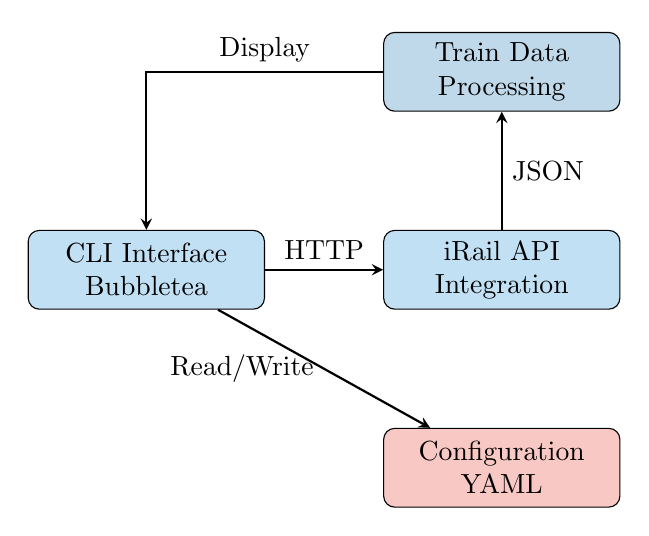
\begin{tikzpicture}[
			node distance=1.5cm,
			box/.style={draw, rounded corners, fill=lightgray, minimum width=3cm, minimum height=1cm, align=center},
			arrow/.style={->, >=stealth, thick}
		]

		\node[box, fill=secondary!30] (cli) {CLI Interface\\Bubbletea};
		\node[box, fill=secondary!30, right=of cli] (api) {iRail API\\Integration};
		\node[box, fill=accent!30, below=of api] (config) {Configuration\\YAML};
		\node[box, fill=primary!30, above=of api] (data) {Train Data\\Processing};

		\draw[arrow] (cli) -- (api) node[midway, above] {HTTP};
		\draw[arrow] (api) -- (data) node[midway, right] {JSON};
		\draw[arrow] (cli) -- (config) node[midway, left] {Read/Write};
		\draw[arrow] (data) -| (cli) node[near start, above] {Display};

	\end{tikzpicture}
\end{center}

\section{Technical Details}
\subsection{Architecture}
The application follows a modular architecture with clear separation of concerns:
\begin{itemize}
	\item \textbf{CLI Layer}: Handles user interaction and command parsing using Cobra
	\item \textbf{API Layer}: Manages communication with the iRail API
	\item \textbf{Data Processing}: Handles JSON parsing and data transformation
	\item \textbf{UI Layer}: Implements the terminal user interface using Bubbletea
	\item \textbf{Configuration}: Manages user preferences and shortcuts using YAML
\end{itemize}

\subsection{Data Flow}
\begin{enumerate}
	\item User input is processed through the CLI interface
	\item Commands are parsed and validated
	\item API requests are made to iRail for relevant data
	\item JSON responses are parsed and transformed
	\item Data is displayed in a formatted table using Bubbletea
	\item User can interact with the displayed information
\end{enumerate}

\section{Challenges \& Solutions}
\subsection{Technical Challenges}
\begin{itemize}
	\item \textbf{API Integration}: Handling various API response formats and error cases
	      \begin{itemize}
		      \item Solution: Implemented robust error handling and JSON parsing
	      \end{itemize}
	\item \textbf{Terminal UI}: Creating an interactive and responsive interface
	      \begin{itemize}
		      \item Solution: Used Bubbletea framework for TUI development
	      \end{itemize}
	\item \textbf{Cross-Platform Compatibility}: Ensuring consistent behavior across different operating systems
	      \begin{itemize}
		      \item Solution: Implemented platform-specific builds using GitHub Actions
	      \end{itemize}
\end{itemize}

\subsection{Lessons Learned}
\begin{itemize}
	\item Importance of proper error handling in CLI applications
	\item Benefits of using modern Go frameworks for TUI development
	\item Value of automated testing and CI/CD pipelines
	\item Need for clear documentation and user guides
\end{itemize}

\section{Screenshots \& Results}
\begin{figure}[h]
	\centering
	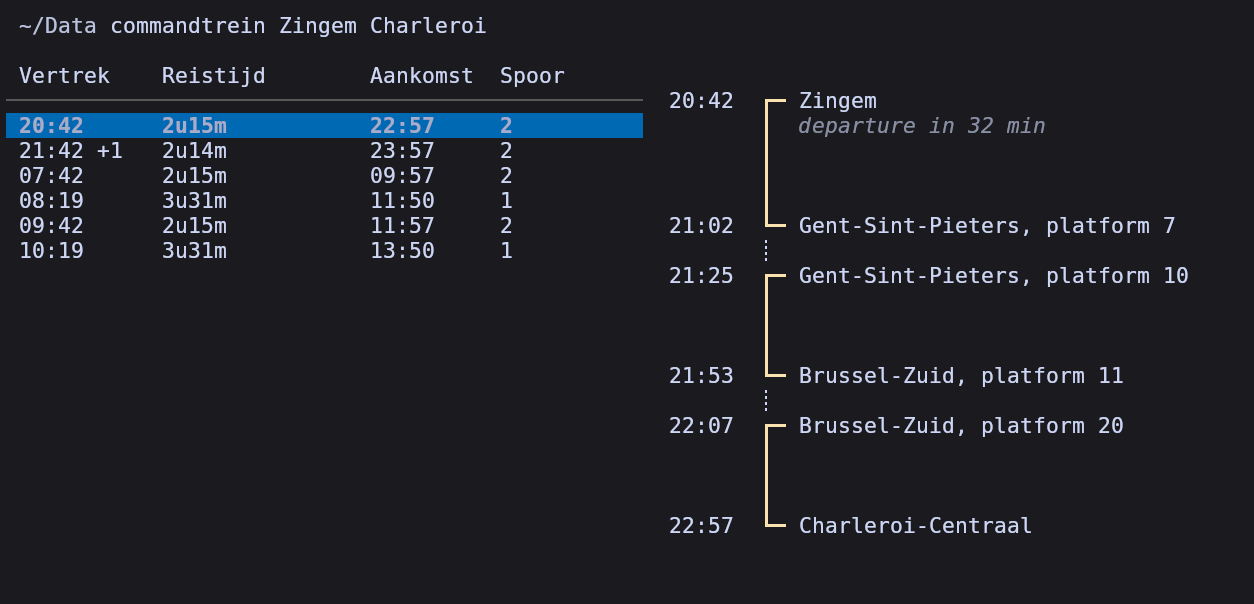
\includegraphics[width=0.8\textwidth]{./images/commandtrein.png}
	\caption{Commandtrein output when asked for connection Zingem - Charleroi}
	\label{fig:screenshot1}
\end{figure}\section{Conclusion}
Commandtrein successfully provides a convenient way to access Belgian train information through the terminal. The project demonstrates effective use of modern Go tooling and frameworks to create a user-friendly CLI application. Future improvements could include:
\begin{itemize}
	\item Enhanced error handling and recovery
	\item Additional customization options
	\item Integration with more transportation services
	\item Offline functionality for basic operations
\end{itemize}

\end{document}
